\section{The groupoid of finite types}~\label{sec:finite}

In this section, we describe \review{the algebraic structure} of the groupoid of
finite types, and give \review{a computable presentation} for it.

\vc{The groupoid of finite types is the free symmetric monoidal groupoid on one
  generator. This can be presented as an algebraic 2-theory, which is our syntax
  for $\PiHatLang$. Vertical categorification of natural numbers as a free
  commutative monoid. See groupoidification.}

\todo{Check Brent Yorgey's thesis?}

To do so, we will characterise the automorphisms on finite sets of cardinality
$n$, and show them to be equivalent to the symmetric group $\Sn$, via the
Coxeter presentation. We will do that in two steps,
in~\cref*{subsec:permutations,subsec:lehmer,subsec:symmetric}.

\todo{Big example: Start from a listed permutation, show Lehmer code, then adjacent swaps.}
\todo{Justification for why we need group theory.}

%% Coxeter presentation of $\Sn$ $\eqv$ $\Lehmer[n]$ $\eqv$ $\Aut[\Fin[n]]$

\subsection{Groups}

From universal algebra, a group is simply a set with a 0-ary constant, the neutral element, a binary operation for group
multiplication, and a unary inverse operation. A simple example is $\mathbb{Z}/n\mathbb{Z}$, where the neutral element
is 0, the inverse of $k$ is $-k$, and the group multiplication is given by addition modulo $n$. The neutral element has
to satisfy unit and inverse laws, and the multiplication has to be associative.

In type theory, a group $G$ can be defined as an $\hSet$ $S$ with the following pieces of data:

\begin{enumerate}
  \item a unit or neutral element $e : S$
  \item a multiplication function $m : S \times S \to S$ written as $(g_{1}, g_{2}) \mapsto g_{1} \mult g_{2}$, that satisfies
  \begin{enumerate}
    \item the unit laws, for all $g : S$, that \( g \mult e \id g \) and \( e \mult g \id g \)
    \item the associativity law, for all $g_{1}, g_{2}, g_{3} : S$, that \( g_{1} \mult (g_{2} \mult g_{3}) \id (g_{1} \mult g_{2}) \mult g_{3} \)
  \end{enumerate}
  \item an inversion function $i : S \to S$ written as $g \mapsto \inv{g}$, that satisfies
  \begin{enumerate}
    \item the inverse laws, for all $g : S$, that \( g \mult \inv{g} \id e \) and \( \inv{g} \mult g \id e \)
  \end{enumerate}
\end{enumerate}

However, more conveniently, in HoTT, we can instead use groupoids to talk about groups. A group can be identified with a
1-object groupoid, using a technique called delooping. The delooping of a group $G$ is a groupoid $\B{G}$ given by a
unique object $\pt$ with self-loops that are 1-paths $\pt \id_{\B{G}} \pt$ corresponding to the elements of $G$. Note
that the group operations are automatically given by operations on the identity type, with $\refl_{\pt}$ for the neutral
element, path composition for the group multiplication, and path inverse for the group inverse. These satisfy the group
laws as well, up to the identity type, using the groupoid coherence laws. Moreover, for 1-groups which are supposed to
be sets, these 2-paths should be propositions, so we have to restrict $\B{G}$ to be a 1-groupoid. Hence, a group is
simply given by a pointed, connected 1-type~\cite*{buchholtzHigherGroupsHomotopy2018,symmetryBook2021}.

For example, given a pointed type $(A:\UU, a:A)$, the automorphism group structure at $a$ is given by $a \id_{A} a$. Of
course, for 1-groups we will require that $a \id_{A} a$ is an $\hSet$, which is enforced by having $A$ be a groupoid. In
our running example for the permutation group on finite sets, we have that $\Fin[n]$ is an $\hSet$, and hence,
$\UFin[n] \defeq \BAut[\Fin[n]]$ is a pointed, connected 1-type, whose loopspace $\loopspace[\BAut[\Fin[n]],F_{n}]$ is
equivalent to $\Aut[\Fin[n]] \defeq (\Fin[n] \eqv \Fin[n]) \eqv (\Fin[n] \id_{\UU} \Fin[n])$, which has the
corresponding automorphism group structure.

\subsection{Free groups}

Given a generating set $A$, we can naively construct a \emph{free group on $A$},
whose elements are drawn from the alphabet $A$, and closed under the group
operations of multiplication and inverse, identified by the group axioms.
For example, the singleton set generates the additive group of integers,
$\mathbb{Z}$.

Usually, there are are many equations, besides the group axioms, that hold for
the elements of the group. For example, in the group $\mathbb{Z}/3\mathbb{Z}$,
we have an equation $1 + 1 + 1 = 0$. A free group has the property that has no
other relations than the ones directly implied by the group axioms.

\todo{What's the best notation for HITs?}
\begin{definition}
  Given an $\hSet$ $A$, the free group $F(A)$ on it is given by a higher
  inductive type with the following point and path constructors. Notice the
  similarity with the definition of a group structure in~\ref{subsec:groups},
  but note that each operation here is a generator for the type $F(A)$\dots.
  \begin{itemize}
    \item An inclusion function $\eta_{A} : A \to F(A)$
    \item A multiplication function $m : F(A) \times F(A) \to F(A)$
    \item An element $e : F(A)$
    \item An inverse function $i : F(A) \to F(A)$
  \end{itemize}
  \smallskip
  \begin{itemize}
    \item For every $x, y, z : F(A)$, a path $\term{assoc} : m(x, m(y, z)) \id m(m(x, y), z)$
    \item For every $x : F(A)$, paths $\term{unitr} : m(x, e) \id x$ and $\term{unitl} : m(e, x) \id x$
    \item For every $x : F(A)$, paths $\term{invr} : m(x, i(x)) \id e$ and $\term{invl} : m(i(x), x) \id e$
    \item A 0-truncation, for every $x, y : F(A)$ and $p, q : x \id y$, a 2-path $\term{trunc} : p \id q$
  \end{itemize}
\end{definition}

A group homomorphism between groups is a function between the underlying sets
that preserves the group structure, which we write as $G_1 \to^G G_2$. With
this, we can state the universal property of free groups.

\begin{proposition}[Universal Property of $F(A)$]~\label{prop:free-groups}
  Given a group $G$ and a map $f : A \to G$, there is a unique group
  homomorphism $\extend{f} : F(A) \to^G G$ such that $\extend{f} \comp \eta_A
  \htpy f$. Equivalently, composition with $\eta_A$ gives an equivalence $F(A)
  \to^G G \eqv A \to G$. Alternatively, the type of group homomorphisms $h :
  F(A) \to^G G$ satisfying $h \comp \eta_A \htpy f$ is contractible.

  % https://q.uiver.app/?q=WzAsMyxbMCwyLCJBIl0sWzAsMCwiRihBKSJdLFsyLDAsIkciXSxbMCwxLCJcXGV0YV9BIl0sWzAsMiwiZiIsMl0sWzEsMiwiXFxleHRlbmR7Zn0iLDAseyJzdHlsZSI6eyJib2R5Ijp7Im5hbWUiOiJkYXNoZWQifX19XSxbMyw0LCJcXGlkIiwwLHsic2hvcnRlbiI6eyJzb3VyY2UiOjIwLCJ0YXJnZXQiOjIwfSwic3R5bGUiOnsiYm9keSI6eyJuYW1lIjoibm9uZSJ9LCJoZWFkIjp7Im5hbWUiOiJub25lIn19fV1d
\[\begin{tikzcd}
	{F(A)} && G \\
	\\
	A
	\arrow[""{name=0, anchor=center, inner sep=0}, "{\eta_A}", from=3-1, to=1-1]
	\arrow[""{name=1, anchor=center, inner sep=0}, "f"', from=3-1, to=1-3]
	\arrow["{\extend{f}}", dashed, from=1-1, to=1-3]
	\arrow["\id", Rightarrow, draw=none, from=0, to=1]
\end{tikzcd}\]
\end{proposition}

This definition of $F(A)$ however has lots of path constructors corresponding to
each group axiom. Alternatively, the free group construction can be thought of
as drawing letters from the generating set, while adding formal inverses, and
constructing words which are sequences of these letters. 

Each element in the sequence can either be an element drawn from the generating
set $a$, or an inverse of such an element $\inv{a}$. If we take the disjoint
union of $A$ with itself, that is, $A + A$ as the underlying set, we can use
$\inl/\inr$ to mark the elements. Hence, we can encode the free group using the
free monoid, that is, lists.

\begin{definition}
  Let $A$ be an $\hSet$, and $\List[\blank]$ the free monoid. The free group
  $F(A)$ on $A$ is the set-quotient of $\List[A + A]$ by the congruence closure
  of the relation $a \cons \inv{a} \cons \nil \sim \nil$.
\end{definition}

\begin{proposition}
  $F(A) \defeq \quot{\List[A + A]}{\sim^{\ast}}$ has a group structure, with the
  empty list $\nil$ for the neutral element, multiplication given by list append
  $\append$, and inverse given by list reversal. Further, $F(A)$ with $\eta_A :
  A \to F(A) \defeq \inl(a) \cons \nil$ satisfies the universal property of free
  groups.~\cref{prop:free-groups}
\end{proposition}

\subsubsection{Group presentations}

One useful way of defining groups is by their presentations. A presentation of a
group builds it by starting from the free group $F(A)$ and introducing a
collection of equations that have to be satisfied in the resulting group. For
example, if we take $F(\unit) \defeq \mathbb{Z}$ and add an equation $1 + 1 + 1
= 0$, the resulting group would be $\mathbb{Z}/3\mathbb{Z}$.

The generators can be thought of as primitive operations in a (reversible)
programming language, group structure gives the way of composing these
operations and inverting them, and relations describe how these primitive
operations interact with each other.

Instead of opereating directly in the semantics of the group operation, here the
focus is on the syntax. While before, the equality of elements (such as the
result of multiplication of two elements) had to be computed externally, now it is
reduced to a \emph{word problem}, i.e., deciding one word can be reduced to another
using group's equations.

However, because equations are not directed, is not always possible to construct a
well-behaving rewriting system. In general, the word problem is proven to be undecidable.

\jk{Example?}

\begin{definition}
  Let $A$ be an $\hSet$ and $R : (A + A) \to (A + A) \to \UU$ a binary relation
  on $A + A$. The group $G$ presented by $\langle A ; R \rangle$ is given by the
  set-quotient of the free group $F(A)$ by the closure of $R$, or equivalently,
  as the coequaliser
  \[\begin{tikzcd}
      FR && FA && G
      \arrow[shift right=2, from=1-1, to=1-3]
      \arrow[shift left=2, from=1-1, to=1-3]
      \arrow[two heads, from=1-3, to=1-5]
    \end{tikzcd}\]
\end{definition}

\vc{do we need this level of detail?}
\todo{Universal property}
\todo{Examples: empty relation, van Kampen of $\pi_{1}$}

The above definition is correct because the universal property of the free group allows 
for properly extending the relation on the generating set to the whole group.
\jk{Turn that into a propostion?}

\subsection{Permutation groups}

Because $\PiLang$ is used for reasoning about reversible functions on finite
sets, the group that we are interested in is the group of permutations on a
fininte set, which is classically know as the symmetric group on $n$ words,
$\Sn$. We've already seen that we can define it formally by taking the
automorphism group given by the type $\Aut[\Fin[n]]$, and showing that it has a
group structure satisfying the group axioms. Alternatively, we can write a group
presentation for $\Sn$ -- by defining a set of generators and a set of relations.

The technical contribution of this section is a proof that these two
descriptions are equivalent. By doing that, we bridge the gap between the
syntactic and semantic notions in our completeness proof -- by establishing a
correspondence between the meaning of a program (a bijection) and its syntax (a
word).

However, in giving a group presentation, there is an element of choice. A group
can be presented in many different ways. For example, we could generate the
permutation group on $\Fin[n]$ by using generators that:

\begin{itemize}
\item swap the $i$-the element with the $(i+1)$-th element, that is, adjacent swaps, or
\item swap the $i$-th element with the $j$-th element, for arbitrary $i$-s and $j$-s, or
\item swap the $i$-th element with an element at a fixed position, or
\item flip a prefix $\Fin[k]$ of $\Fin[n]$ for $k \leq n$, or
\item cyclically shift any subset of $\Fin[n]$.
\end{itemize}

One way of thinking about these presentations is via sorting algorithms, which
use different primitive operations. A sorting algorithm has to calculate a
permutation of a list or a finite set, which satisfies the invariant of being a
sorted sequence, which means, the primitive operations of a sorting algorithm
should be able to generate all the permutations on a given list. If using a
chosen set of reversible operations, one can write a sorting algorithm, then
those operations generate the permutation group.

For example, bubble sort uses the primitive operation of adjacent swaps,
insertion sort and selection sort use the primitive operation of swapping the
$i$-th element with the $j$-th element, cycle sort uses cyclical shifts of
subsequences, pancake sort uses flips of prefixes of the list, et cetera.
\todo{check!}

\subsection{Coxeter Presentation}

To do the proof, we are using a presentation based on the adjacent
transpositions, i.e. where the primitive operations are adjacent swaps. There
are three laws that these operations have to satisfy - it is easiest to
visualize them on diagrams.
\begin{itemize}
\item Swapping the same two elements two times in a row is the same as doing nothing:
    \begin{tikzpicture}
        \pic[local bounding box=my braid,braid/.cd, 
        number of strands = 2,
        thick]
        {braid={ s_1, s_1}};
    \end{tikzpicture}
    \hspace{1cm}
    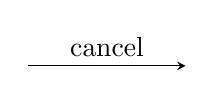
\begin{tikzpicture}
        \draw [-stealth](0,0) -- node[anchor=south] {cancel} (2,0);
    \end{tikzpicture}
    \hspace{1cm}
    \begin{tikzpicture}
        \pic[local bounding box=my braid,braid/.cd, 
        number of strands = 2,
        thick]
        {braid={1, 1}};
    \end{tikzpicture}
\item When swapping two pairs of elements on a positions far away, it does not
matter in which order it is done (We can slide the wires).
    \begin{tikzpicture}
        \pic[local bounding box=my braid,braid/.cd, 
        number of strands = 2,
        thick]
        {braid={ 1, s_1}};
    \end{tikzpicture}
    \hspace{0cm}
    \dots
    \hspace{0cm}
    \begin{tikzpicture}
        \pic[local bounding box=my braid,braid/.cd, 
        number of strands = 2,
        thick]
        {braid={ s_1, 1 }};
    \end{tikzpicture}
    \hspace{1cm}
    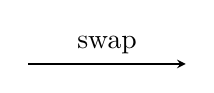
\begin{tikzpicture}
        \draw [-stealth](0,0) -- node[anchor=south] {swap} (2,0);
    \end{tikzpicture}
    \hspace{1cm}
    \begin{tikzpicture}
        \pic[local bounding box=my braid,braid/.cd, 
        number of strands = 2,
        thick]
        {braid={ s_1, 1}};
    \end{tikzpicture}
    \hspace{0cm}
    \dots
    \hspace{0cm}
    \begin{tikzpicture}
        \pic[local bounding box=my braid,braid/.cd, 
        number of strands = 2,
        thick]
        {braid={ 1, s_1}};
    \end{tikzpicture}

\item seen on a diagram (braid)
    \begin{tikzpicture}
        \pic[local bounding box=my braid,braid/.cd, 
        number of strands = 3,
        thick]
        {braid={ s_2, s_1, s_2}};
    \end{tikzpicture}
    \hspace{1cm}
    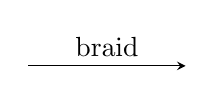
\begin{tikzpicture}
        \draw [-stealth](0,0) -- node[anchor=south] {braid} (2,0);
    \end{tikzpicture}
    \hspace{1cm}
    \begin{tikzpicture}
        \pic[local bounding box=my braid,braid/.cd, 
        number of strands = 3,
        thick]
        {braid={ s_1, s_2, s_1}};
    \end{tikzpicture}

\end{itemize}

Diagram of long-braid:
\begin{tikzpicture}
    \pic[local bounding box=my braid,braid/.cd, 
    number of strands = 2,
    thick]
    {braid={1, 1, 1, 1, s_1, 1}};
\end{tikzpicture}
\hspace{0cm}
\dots
\hspace{0cm}
\begin{tikzpicture}
    \pic[local bounding box=my braid,braid/.cd, 
    number of strands = 5,
    thick]
    {braid={ s_4, s_3, s_2, s_1, 1, s_4}};
\end{tikzpicture}
\hspace{1cm}
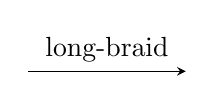
\begin{tikzpicture}
    \draw [-stealth](0,0) -- node[anchor=south] {long-braid} (2,0);
\end{tikzpicture}
\hspace{1cm}
\begin{tikzpicture}
    \pic[local bounding box=my braid,braid/.cd, 
    number of strands = 2,
    thick]
    {braid={1, 1, 1, 1, 1, s_1}};
\end{tikzpicture}
\hspace{0cm}
\dots
\hspace{0cm}
\begin{tikzpicture}
    \pic[local bounding box=my braid,braid/.cd, 
    number of strands = 5,
    thick]
    {braid={ s_3, s_4, s_3, s_2, s_1, 1}};
\end{tikzpicture}
\hspace{1cm}


This construction is called a Coxeter presentation. Writing it formally, we
get the following definition
Definition: Coxeter presentation.

13. There are two main considerations to this choice:
13a. How well the presentation matches the syntactic side of Pi? This is,
how closely does the operational semantics built from these particular
primitive operations match the natural operational semantics of Pi?
13b. How convenient is it to turn the presentation it into rewriting system
and solve the word problem for it?

Thus, the argument:
14. TODO I don't know what to write here, we have to think.

15a. The equations that define Coxeter presentation have a nice property:
as it is written, the LHS is smaller (lexicographically) than the RHS.
Thus, if we could direct them from right to left, it would have a
termination property out of the box.
15b. However, it is not at all obvious that the system would be confluent.
There are many possible critical pairs, such as
TODO diagram 1212 (braid, braid)
or
TODO diagram 3233 (braid, cancel)
As it turns out, there are instances of critical pairs that do not resolve.
A simplest example is the following:
TODO diagram 3213

16. The equations have to be changed. We thus propose a new presentation.
We keep the (cancel) and (swap) equations, but replace (braid) with a more
general:
TODO diagram:

Definition: Long Coxeter presentation.

17. In return for increased complexity of the equations, it satisfies the
diamond property (if we direct the equation). Thus, together with the
(preserved) termination, it creates a confluent rewriting system.
Proof: All the critical pairs resolve, in the appendix.
Definition: A normal form is a list that cannot be reduced any further.

18. We define the equivalence classes on List (Fin n) to be precisely these
elements that have the same normal form.

19. However, the Long Coxeter relations are unwieldly and have no
connectino to the broader scope of computational group theory - while the
usual Coxeter presentation is to-go choice in this area (cite all these
papers in Coq, this guy from Sweden(?) etc.).
Thus, we prove:
Proposition: Long Coxeter is equivalent to normal Coxeter.

19a. (Note: here we try to convince the reader about reusability badge) So,
the Long Coxeter can be regarded as a trick to get the proof to pass - but
the external user-facing interface is still that of the usual Coxeter
presentation.

20. Now, to prove the equivalence of 9, on one side we have Aut(Fin n), and
on the other, equivalence classes of List (Fin n) wrt to the usual Coxeter
group, we would define two functions from and back. The easiest way to
define a function out of the group presentation is to define them on the
equivalence classes' representatives. But to do that, we have to know how
do these representatives look like exactly.

\subsection{Lehmer Codes}

21. Enter: Lehmer codes.
TODO diagram with List (Fin n) being divided into equivalence classes, and
Lehmer codes being an image of immersion, being the normal form
(representative) in each class.

\subsection{Permutations}~\label{subsec:permutations}

In the previous~\cref{sec:univalent}, we established that paths in $\UFin$ are
equivalent to families of automorphisms of $\Fin{n}$ for every $n:\Nat$, that
is, bijections on finite sets of size $n$. This is the extensional view of
permutations. In the following sections, we will characterise these
permutations, going through two intermediate steps.

\vc{This is obvious, maybe add something more here.}

\subsection{Lehmer codes}~\label{subsec:lehmer}

From grade school combinatorics, we know that there are $\fac{n}$ permutations
on a finite set with $n$ elements. The factorial function is defined by
recursion on natural numbers. However, now, for every $n$, we want to produce a
type, which is a finite set, with cardinality $\fac{n}$. And, to characterise
$\Aut[\Fin[n]]$, we further need to construct a bijection between this type and
$\Aut[\Fin[n]]$.

First, let's define this type with $\fac{n}$ elements, we name this type family
$\Lehmer : \Nat \to \UU$, which is defined by recursion on $\Nat$ as follows.
This is the obvious definition of factorials by recursion, but categorified from
natural numbers to sets.

\begin{definition}
  \begin{align*}
    \Lehmer[0]       & \defeq \unit                           \\
    \Lehmer[\suc[n]] & \defeq \Fin[\suc[n]] \times \Lehmer[n]
  \end{align*}
\end{definition}

\todo{Subexcedant sequences and factorial definitions are equivalent, explain
  this!}

The name Lehmer comes from Lehmer
codes~\cite{lehmerTeachingCombinatorialTricks1960} which are known in
Combinatorial Analysis~\cite{bellmanCombinatorialAnalysis1960}. There are many
ways to represent permutations, e.g. inversions, or cycles, or matrices. Lehmer
codes are a particularly convenient way to represent permutations on a
computer,~\review{they are compact and have exactly the right cardinality.
  $\Lehmer[n]$ is a $n+1$-element tuple, where the position $k \leq n$ has an
  element of $\Fin[k]$. The 0-th position is trivial, so we ignore it, and in
  both the example below and the Agda proof, consider only the remaining
  $n$-element tuple.}

\vc{This is just the classical algorithm to explain the example, not the actual
  type-theoretic proof.}

Suppose we have a permutation $p$ on an $n$-element set
$\{\el{0}, \el{1}, \el{2}, \el{3}, \el{4}\}$, we encode it as follows.
$\Lehmer[n]$ is a $n$-element tuple. At position $k$, we put the number of
inversions of the element $\el{k}$ in $p$, i.e. the number of elements smaller
than $\el{k}$ occurring after $\el{k}$.

As an example, consider the following tabulated presentation of the permutation:

\todo{fix this figure}

\[
  p =
  \begin{array}{ccccccccccccccc}
    | & 0      & | & 1      & | & 2      & | & 3      & | & 4      & | \\
    \hline                                                             \\
    | & \el{2} & | & \el{0} & | & \el{1} & | & \el{4} & | & \el{3} & | \\
    \hline                                                             \\
  \end{array}
\]

%  0 1 2 3 4
% -----------
% |2|0|1|4|3|
% -----------

The element $\el{0}$ has 0 inversions, because there are no elements smaller
than $\el{0}$ occurring after it. In fact, there can be no elements smaller than
$\el{0}$ at all, so the type at the first position of the Lehmer code tuple is
$\unit$.

The element $\el{1}$ has 0 inversions as well, since elements occurring after it
in the permutation are $\el{4}$ and $\el{2}$. There is only one different case,
if $\el{1}$ appeared before $\el{0}$, it would have 1 inversion. This is why the
type of the second component of the Lehmer code is $\Fin[2]$.

The element $\el{2}$ has 2 inversions, because both $\el{0}$ and $\el{1}$ occur
after it in the permutation. The element $\el{3}$ occurs as the last one, so it
has 0 inversions. The element $\el{4}$ has 1 inversion, with the element
$\el{3}$.

Thus, the Lehmer code for the permutation $p$ is the 5-tuple
$l = (0, 0, 2, 0, 1)$.

To reconstruct the tabulated presentation of the permutation from the Lehmer
code, we perform an algorithm similar to \emph{insertion sort}. Starting from
the left-most position of the tuple $l$, we'll read the value $v$, insert the
new element at the end of the newly created list, and shift it backward $v$
places.

\begin{center}
  \begin{tabular}{c|p{0.75\linewidth}}
    (0, 0, 2, 0, 1)               & We start from an empty list $[]$                                                                 \\
    (\highlight{{0}}, 0, 2, 0, 1) & We read 0 as the left-most value from $l$. Thus, we append the element $\el{0}$ to our
                                    list, getting $[\el{0}]$. The element is shifted $0$ places, so it remains in the
                                    same place.                                                                                                                      \\
    (0, \highlight{{0}}, 2, 0, 1) & Then, similarly, we read another 0 for the element $\el{1}$, append it to the
                                    list getting $[\el{0}, \el{1}]$, and don't shift it either.                                                                      \\
    (0, 0, \highlight{{2}}, 0, 1) & We read 2 for the next the element $\el{2}$ - we append $\el{2}$ to our list, getting
                                    $[\el{0}, \el{1}, \el{2}]$, and shift it 2 places right, which results in a list $[\el{0}, \el{2}, \el{1}]$
                                    \todo{Typeset it nicely, with arrows showing the shifting}.                                                                      \\
    (0, 0, 2, \highlight{{0}}, 1) & Then we read 0 - appending $\el{3}$ and not shifting, getting $[\el{0}, \el{2}, \el{1}, \el{3}]$ \\
    (0, 0, 2, 0, \highlight{{1}}) & Finally, reading 1 for element $\el{4}$ - appending $\el{4}$ to the list and shifting it
                                    one place right results in the final list $[\el{0}, \el{2}, \el{1}, \el{4}, \el{3}]$                                             \\
  \end{tabular}
\end{center}
\todo{figure}

Using this Lehmer encoding algorithm, we can now construct the equivalence between these types.

We define a type family $\FinExcept{n} : \Fin[n] \to \UU$ which picks out all elements in $\Fin[n]$ except the one
provided. Note that $\FinExcept{n}[i]$ for $i : \Fin[n]$ is a subtype of $\Fin[n]$ and is hence an $\hSet$.

\begin{definition}
  \( \FinExcept{n}[i] \defeq \dsum{j : \Fin[n]}{i \neq j} \).
\end{definition}

\begin{proposition}
  For any $k : \Fin[n]$, $\unit \sqcup \FinExcept{n}[k] \eqv \Fin[n]$.
\end{proposition}

\begin{proposition}
  For any $k : \Fin[\suc[n]]$, $\FinExcept{\suc[n]}[k] \eqv \Fin[n]$.
\end{proposition}

\begin{proposition}
  For any $n : \Nat$,
  \( \Aut[\Fin[\suc[n]]] \eqv \dsum{k : \Fin[\suc[n]]}{\FinExcept{\suc[n]}[\fzero] \eqv \FinExcept{\suc[n]}{k}} \).
\end{proposition}

\begin{proposition}
  For all $n:\Nat$, \( \Lehmer[n] \eqv \Aut[\Fin[n]] \).
\end{proposition}

\begin{proof}
  For $n = 0$, note that $\Lehmer[0]$ is contractible, and so is $\Aut[\Fin[0]]$. For $n = \suc[m]$, we have the
  following chain of equivalences.
  \[\arraycolsep=0.5em\def\arraystretch{1.5}
    \begin{array}{rl}
      & \Aut[\Fin[\suc[m]]] \\
      \eqv & \dsum{k : \Fin[\suc[m]]}{\FinExcept{\suc[m]}[\fzero] \eqv \FinExcept{\suc[m]}[k]} \\
      \eqv & \dsum{k : \Fin[\suc[m]]}{\FinExcept{\suc[m]}[\fzero] \eqv \Fin[m]} \\
      \eqv & \dsum{k : \Fin[\suc[m]]}{\Fin[m] \eqv \Fin[m]} \\
      \eqv & \Fin[\suc[m]] \times \Aut[\Fin[m]] \\
      \eqv & \Fin[\suc[m]] \times \Lehmer[m] \\
    \end{array}
  \]
\end{proof}

\subsection{Symmetric groups}~\label{subsec:symmetric}

There is an obvious group structure on $\Aut[\Fin[n]]$ given by identity,
composition, and inverse. This is the symmetric group $S_n$ on $n$ symbols. In
the rest of the section we will construct a convenient presentation of this
group.

\vc{this is just a rough draft for now}

\todo{Reference T-algebra presentations as coequalisers (Mac Lane 6.7)}

First, we formally define a presentation of a group.

\todo{Free 1-group, needs to be truncated}


\subsubsection{Coxeter Relations}

We define a binary relation on $\List[\Fin[n]]$.

\begin{definition}[$\cox$]
  \begin{align*}
    \cancel
    & : \forall n \to (n \cons n \cons \nil) \cox \nil \\
    \swap
    & : \forall k, n \to (\suc[k] < n) \to (n \cons k \cons \nil) \cox (k \cons n \cons \nil) \\
    \braid
    & : \forall n \to (\suc[n] \cons n \cons \suc[n] \cons \nil) \cox (n \cons \suc[n] \cons n \cons \nil) \\
  \end{align*}
\end{definition}

We define $\cox*$ as the congruence closure of $\cox$.
\vc{This could be simplified a bit depending on our formalisation. $\cox$ is directed, use a different symbol?}

\begin{definition}[$\cox*$]
  \begin{align*}
    \reflr{\cox}
    & : \forall w \to w \cox* w \\
    \symr{\cox}
    & : \forall w_{1}, w_{2} \to w_{1} \cox* w_{2} \to w_{2} \cox* w_{1} \\
    \transr{\cox}
    & : \forall w_{1}, w_{2}, w_{3} \to  w_{1} \cox* w_{2} \to w_{2} \cox* w_{3} \to w_{1} \cox* w_{3} \\
    \congrf{\cox}{\append}
    & : \forall w_{1}, w_{2}, w_{3}, w_{4} \to  w_{1} \cox* w_{2} \to w_{3} \cox* w_{4} \to w_{1} \append w_{3} \cox* w_{2} \append w_{4} \\
    \relr{\cox}
    & : \forall w_{1}, w_{2} \to w_{1} \cox w_{2} \to w_{1} \cox* w_{2} \\
  \end{align*}
\end{definition}

\todo{Long form of Coxeter relations and their equivalence.}

We state and prove two desirable properties of this relation on $\List[\Fin[n]]$ from the point of view of an abstract
rewriting system. We follow the terminology of~\cite{krausCoherenceWellFoundednessTaming2020}. \vc{Not completely
  formalised. Is this with Coxeter or LongCoxeter?}

\begin{proposition}
  \leavevmode
  \begin{enumerate}
    \item $\cox$ is (locally) confluent. For every span $w_{1} \cox w \cox w_{2}$, there is a matching extended cospan
          $w_{1} \cox* v \cox* w_{2}$.
    \item $\cox*$ is strongly normalising. For every $w$, there exists a unique $v$ such that $w \cox* v$.
          \review{Equivalently, the type $\dsum{v:\List[\Fin[n]]}{w \cox* v}$ is contractible, and $w \cox* v$ is a
          proposition for every $w$ and $v$.}
  \end{enumerate}
\end{proposition}

The type $\Sn$ is defined as the set-quotient of $\List[\Fin[n]]$ by $\cox*$.

\begin{definition}[$\Sn$]
  \(\Sn \defeq \quot{\List(\Fin[n])}{\cox*}\)
\end{definition}

We will now prove the group structure of $\Sn$.

\begin{proposition}
  There is a group structure on $\Sn$, where the identity element is $\nil$, multiplication is given by list append, and
  inverse is given by list reversal.
\end{proposition}

\begin{proposition}
  $\Sn$ is equivalent to the generated group given by the normal closure of $\cox*$ extended to
  $\List(\Fin[n] + \Fin[n])$ along the codiagonal map $[\term{id},\term{id}] : A + A \to A$.
\end{proposition}

We will now show how to generate a Lehmer code from a word in $\Sn$ and back.

\begin{definition}
  \[
    \encode{\List} : \List[\Fin[n]] \to \Lehmer[n]
  \]
\end{definition}

\begin{proposition}
  \leavevmode
  \begin{enumerate}
    \item \( l_{1} \cox* l_{2} \to \encode{\List}(l_{1}) \id \encode{\List}(l_{1}) \)
  \end{enumerate}
\end{proposition}

\begin{definition}
  \begin{align*}
    \encodeSn & : \Sn[n] \to \Lehmer[n] \\
    \decodeSn & : \Lehmer[n] \to \Sn[n]
  \end{align*}
\end{definition}

\begin{proposition}
  For all $n : \Nat$, $(\encodeSn, \decodeSn)$ is an equivalence.
\end{proposition}

\begin{corollary}
  For all $n : \Nat$,
  \(
    \Sn \eqv \Lehmer[n] \eqv \Aut[\Fin[n]]
  \).
\end{corollary}

%%% Local Variables:
%%% mode: latex
%%% TeX-master: "main"
%%% fill-column: 120
%%% End:
